\documentclass{beamer}
\usepackage{alltt}
\usepackage{tikz}
\usetikzlibrary{matrix}
\usetikzlibrary{trees}
\usepackage{cancel}
\usepackage{subcaption}
\PassOptionsToPackage{obeyspaces}{url}
\usepackage{hyperref}
\usepackage{adjustbox}

\usepackage{lipsum}

\usetheme{Hannover}

\newcommand{\racket}{\texttt{Racket}}
\newcommand{\drr}{\texttt{DrRacket}}
\newcommand{\fsm}{\texttt{FSM}}
\newcommand{\ide}{\texttt{IDE}}
\newcommand{\api}{\texttt{API}}
\newcommand{\arrow}{\(\rightarrow\)}
\newcommand{\dotss}{\(\ldots\)}
\newcommand{\vdotss}{\(\vdots\)}
\newcommand{\elist}{\texttt{\textquotesingle{()}}}
\newcommand{\logand}{\texttt{\(\wedge\)}}
\newcommand{\logor}{\texttt{\(\vee\)}}
\newcommand{\imp}{\texttt{\(\Rightarrow\)}}
\newcommand{\sig}{\texttt{\(\Sigma\)}}
\newcommand{\delt}{\texttt{\(\delta\)}}
\newcommand{\sigsig}{\texttt{\(\Sigma\) = \{a b\}}}
\newcommand{\gam}{\texttt{\(\Gamma\)}}
\newcommand{\ep}{\texttt{\(\epsilon\)}}
\newcommand{\quot}{\texttt{\textquotesingle{}}}
\newcommand{\dquot}{\texttt{"}}
\newcommand{\qquot}{\texttt{\textasciigrave{}}}
\newcommand{\lambexpr}{\texttt{$\lambda$}-expression}
\newcommand{\lamb}{\texttt{$\lambda$}}
\newcommand{\is}{\texttt{::=}}

\definecolor{darkgreen}{RGB}{102,170,102}

\begin{document}

\title{Part I: Introduction}
%\subtitle{Using Beamer}
\author{Marco T. Moraz\'{a}n}
\institute{Seton Hall University}
\date{}

\begin{frame}
\titlepage
\end{frame}

\begin{frame}
\frametitle{Outline}
\tableofcontents
\end{frame}

\section{Introduction}

\begin{frame}[fragile]
\frametitle{Recursively Specified Data}
%\framesubtitle{HOMEWORK}
\begin{scriptsize}
\begin{itemize}
\item<1-> When writing a function we must know precisely what kinds of values may occur as arguments

\item<2-> Data of arbitrary size requires an inductive data definition

\item<2-> To specify a set, S, inductively, define it as the smallest set satisfying two properties:
  \begin{itemize}
    \item<2-> Some specific values are in S
    \item<2-> If certain values are in S, then certain other values are in S
  \end{itemize}

\item<3->
  \begin{itemize}
    \item<2-> 0$\in$S
    \item<2-> x+3$\in$S, where x$\in$S
  \end{itemize}

\item<3-> What has been defined?

\end{itemize}
\end{scriptsize}
\end{frame}

\begin{frame}[fragile]
\frametitle{Introduction}
%\framesubtitle{HOMEWORK}
\begin{scriptsize}
\begin{itemize}
\item<1-> Data of arbitrary size can also be defined using inference rules

\item<2->
  \begin{itemize}
    \item<2-> $\frac{}{0\in{}S}$\newline \\

    \item<2-> $\frac{x\in{}S}{x+3\in{}S}$
  \end{itemize}

\item<3-> Define a list of numbers

\item<4->
  \begin{itemize}
    \item $\frac{}{\elist{}\in{}(listof number)}$\newline \\

    \item $\frac{L\in{}(listof number)}{(cons number L)\in{}S}$
  \end{itemize}

\end{itemize}
\end{scriptsize}
\end{frame}

\begin{frame}[fragile]
\frametitle{Introduction}
%\framesubtitle{HOMEWORK}
\begin{scriptsize}
\begin{itemize}
\item<1-> A third way to specify data is using \texttt{BNF} (Backus Naur Form)

\item<1-> Grammar rules used to specify programming languages

\item<2-> Elements of rules
  \begin{description}
    \item[Terminal symbols] Characters in the external representation \newline
    \item[Nonterminal Symbols] Names of sets being defined usually in angle brackets (syntactic categories) \newline
    \item[Productions] Rules with a RHS and a LHS
      \begin{itemize}
        \item LHS \is{} RHS \newline
        \item Read as: LHS can be/is RHS
      \end{itemize}
\end{description}


\end{itemize}
\end{scriptsize}
\end{frame}

\begin{frame}[fragile]
\frametitle{Introduction}
%\framesubtitle{HOMEWORK}
\begin{scriptsize}
\begin{itemize}
\item<1-> List of numbers
  \begin{itemize}
    \item $<$lon$>$ \is{} \elist{} \newline
    \item $<$lon$>$ \is{} (cons $<$number$>$ $<$lon$>$)
  \end{itemize}

\item<2-> Syntactic Derivation: (2 4)
  \begin{tabular}{lll}
    %\hline
    % after \\: \hline or \cline{col1-col2} \cline{col3-col4} ...
    $<$lon$>$ & \is{} & ($<$number$>$  $<$list-of-numbers$>$) \\
     & \is{} & (2  $<$list-of-numbers$>$) \\
     & \is{} & (2  $<$number$>$ $<$list-of-numbers$>$) \\
     & \is{} & (2  4 $<$list-of-numbers$>$) \\
     & \is{} & (2  4) \\
    %\hline
  \end{tabular}

\item<2-> Order of substitutions does not matter

\end{itemize}
\end{scriptsize}
\end{frame}

\begin{frame}[fragile]
\frametitle{Introduction}
%\framesubtitle{HOMEWORK}
\begin{scriptsize}
\begin{itemize}
\item<1-> Symbolic Lists

\item<1->
\begin{itemize}
    \item $<$slist$>$ \is{} ($<$sexp$>^*$) \newline
    \item $<$sexp$>$ \is{} $<$symbol$> | <$slist$>$)
\end{itemize}

\item<2-> Derivation of (a (b c) d)

\item<2->
  \begin{tabular}{lll}
    %\hline
    % after \\: \hline or \cline{col1-col2} \cline{col3-col4} ...
    $<$slist$>$ & \is{} & ($<$sexp$>^*$) \\
     & \is{} & ($<$sexp$>$ $<$sexp$>$ $<$sexp$>$) \\
     & \is{} & (a  $<$sexp$>$ $<$sexp$>$) \\
     & \is{} & (a $<$sexp$>$ d) \\
     & \is{} & (a $<$slist$>$ d) \\
     & \is{} & (a ($<$sexp$>^*$) d)\\
     & \is{} & (a ($<$sexp$>$ $<$sexp$>$) d)\\
     & \is{} & (a (b $<$sexp$>$) d)\\
     & \is{} & (a (b c) d)\\
    %\hline
  \end{tabular}
\end{itemize}
\end{scriptsize}
\end{frame}

\begin{frame}[fragile]
\frametitle{Introduction}
%\framesubtitle{HOMEWORK}
\begin{scriptsize}
\begin{itemize}
\item<1-> Define a binary tree with numeric leaves
\item<1->
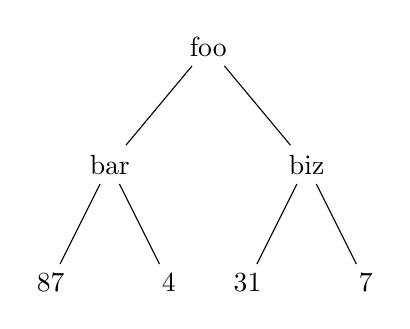
\begin{tikzpicture}
\node {foo}[sibling distance = 2.5cm]
    child {node {bar}[sibling distance = 1.5cm]
      child {node {87}}
      child {node {4}}}
    child {node {biz}[sibling distance = 1.5cm]
      child {node {31}}
      child {node {7}}};
\end{tikzpicture}

\item<2->
\begin{itemize}
    \item $<$bintree$>$ \is{} $<$number$>$ \newline
    \item $<$bintree$>$ \is{} ($<$symbol$>$ $<$bintree$>$ $<$bintree$>$)
\end{itemize}
\end{itemize}
\end{scriptsize}
\end{frame}

\begin{frame}[fragile]
\frametitle{Introduction}
%\framesubtitle{HOMEWORK}
\begin{scriptsize}
\begin{itemize}
\item<1-> The Lambda Calculus

\item<1-> A simple language used to study the theory of programming languages

\item<1-> Contains:
  \begin{itemize}
    \item variable references
    \item lambda expressions with a single parameter
    \item application expressions
  \end{itemize}

\item<2->
  \begin{tabular}{lll}
    %\hline
    % after \\: \hline or \cline{col1-col2} \cline{col3-col4} ...
    $<$exp$>$ & \is{} & $<$id$>$ \\
     & \is{} & (lambda ($<$id$>$) $<$exp$>$) \\
     & \is{} & ($<$exp$>$ $<$sexp$>$) \\
    %\hline
  \end{tabular}

\end{itemize}
\end{scriptsize}
\end{frame}

\begin{frame}[fragile]
\frametitle{Introduction}
%\framesubtitle{HOMEWORK}
\begin{scriptsize}
\begin{itemize}
\item<1-> HOMEWORK: 1.1, 1.3

\end{itemize}
\end{scriptsize}
\end{frame}

\begin{frame}[fragile]
\frametitle{Introduction}
%\framesubtitle{HOMEWORK}
\begin{scriptsize}
\begin{itemize}
\item<1-> BNF grammars are also known as context-free grammars

\item<1-> Rules may be used regardless of the context in any order

\item<2-> Not all sets are context-free

\item<2-> Consider defining the set of BSTs of numbers

\item<2->
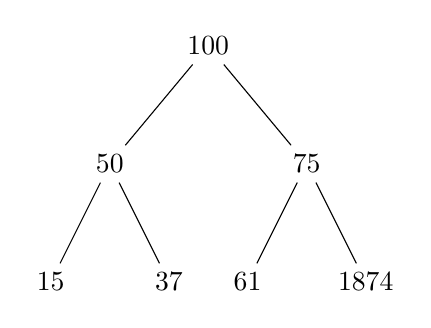
\begin{tikzpicture}
\node {100}[sibling distance = 2.5cm]
    child {node {50}[sibling distance = 1.5cm]
      child {node {15}}
      child {node {37}}}
    child {node {75}[sibling distance = 1.5cm]
      child {node {61}}
      child {node {1874}}};
\end{tikzpicture}

\item<3->
  \begin{tabular}{lll}
    %\hline
    % after \\: \hline or \cline{col1-col2} \cline{col3-col4} ...
    $<$bst$>$ & \is{} & \elist{} \\
     & \is{} & ($<$number$>$ $<$bst$>$ $<$bst$>$) \\
    %\hline
  \end{tabular}

\item<3-> Any problems with this?

\item<4-> Does not capture: everything in the LST must be $\leq$ to the root number and everything in the RST

\item<4-> Such constraints are context-sensitive: valid LSTs and RSTs depend on the root value

\item<5-> Arise in some PLs: variables must be declared before using them

\end{itemize}
\end{scriptsize}
\end{frame}

\begin{frame}[fragile]
\frametitle{Introduction}
%\framesubtitle{HOMEWORK}
\begin{scriptsize}
\begin{itemize}
\item<1-> Proving properties of recursive data is done using induction

\item<2-> Prove that T$\in$\texttt{bintree} $\imp{}$ T has an odd number of nodes

\item<3-> Proof by induction on, h, the height of T

\item<3-> Base case: h = 0
\begin{alltt}
h = 0 \(\imp{}\) T is a number
      \(\imp{}\) T has one node
      \(\imp{}\) T has an odd number of nodes
\end{alltt}

\item<4-> Inductive case
\begin{alltt}
Assume: T has an odd number for nodes for h = k
Prove: T has an odd number for nodes for h = k+1

h = k+1 \(\imp{}\) T is not a number
        \(\imp{}\) T has a root number and two sub-bintrees: lst and rst

Both lst and rst have height at most k
  \(\imp{}\) each has an odd number of nodes (by IH)
  \(\imp{}\) lst has 2*i+1 nodes and rhs has 2*j+1 nodes
  \(\imp{}\) T has 2*i+1 + 2*j+1 + 1 nodes = 2(i+j)+3 nodes
  \(\imp{}\) T has an odd number of nodes \(\qed\)
\end{alltt}

\end{itemize}
\end{scriptsize}
\end{frame}

\begin{frame}[fragile]
\frametitle{Introduction}
%\framesubtitle{HOMEWORK}
\begin{scriptsize}
\begin{itemize}
\item<1-> Write a program to count the number of nodes in a bintree

\item<2->
\begin{tabular}{lll}
    %\hline
    % after \\: \hline or \cline{col1-col2} \cline{col3-col4} ...
    $<$bst$>$ & \is{} & \elist{} \\
     & \is{} & ($<$number$>$ $<$bst$>$ $<$bst$>$) \\
    %\hline
\end{tabular}

\item<3->
\begin{alltt}
#lang eopl
(require rackunit)
#|
bintree \is{} number
        \is{} (number bintree bintree)
|#
\end{alltt}

\item<4->
\begin{alltt}
;; bintree \arrow{} odd-natnum
;; Purpose: Count the nodes the given bintree
(define (cnt-nodes s)
\end{alltt}

\item<6->
\begin{alltt}
  (if (number? s)
      1
\end{alltt}

\item<7->
\begin{alltt}
      (+ 1 (cnt-nodes (cadr s)) (cnt-nodes (caddr s)))))
\end{alltt}

\item<5->
\begin{alltt}
(check-equal? (cnt-nodes 23) 1)
(check-equal? (cnt-nodes (list 45 88 6561)) 3)
(check-equal? (cnt-nodes (list 45 (list 88 11 99)
                                  (list 6561 -6 42)))
              7)
\end{alltt}

\end{itemize}
\end{scriptsize}
\end{frame}

\begin{frame}[fragile]
\frametitle{Introduction}
%\framesubtitle{HOMEWORK}
\begin{scriptsize}
\begin{itemize}
\item<1-> \textbf{Follow the Grammar}

\item<1-> At least one function for each syntactic category (i.e., nonterminal)

\item<1-> Processing an instance of a syntactic category is done by calling a function to process instances of the syntactic category

\end{itemize}
\end{scriptsize}
\end{frame}

\begin{frame}[fragile]
\frametitle{Introduction}
%\framesubtitle{HOMEWORK}
\begin{scriptsize}
\begin{itemize}
\item<1-> Write a predicate of a lon

\item<1->
\begin{itemize}
    \item $<$lon$>$ \is{} \elist{} \newline
    \item $<$lon$>$ \is{} (cons $<$number$>$ $<$lon$>$)
\end{itemize}

\item<2->
\begin{alltt}
#lang eopl
(require rackunit)

#|
lon ::= ()
    ::= (number lon)
|#
\end{alltt}

\item<3->
\begin{alltt}
;; (listof X) \arrow Boolean
;; Purpose: Determine if the given input is a lon
(define (lon? l)
\end{alltt}

\item<5->
\begin{alltt}
  (if (null? l)
      #t
\end{alltt}

\item<6->
\begin{alltt}
      (and (number? (car l)) (lon? (cdr l)))))
\end{alltt}

\item<4->
\begin{alltt}
(check-equal? (lon? \quot{}(a b c d)) #f)
(check-equal? (lon? \elist{}) #t)
(check-equal? (lon? \quot{}(1 2 3)) #t)
\end{alltt}

\end{itemize}
\end{scriptsize}
\end{frame}

\begin{frame}[fragile]
\frametitle{Introduction}
%\framesubtitle{HOMEWORK}
\begin{scriptsize}
\begin{itemize}
\item<1->
\begin{alltt}
;; (listof X) \arrow Boolean
;; Purpose: Determine if the given list is a lon
(define (lon? l)
  (if (null? l)
      #t
      (and (number? (car l)) (lon? (cdr l)))))
\end{alltt}

\item<2-> Prove that the function is correct

\item<3-> Proof by induction on, k, $|$l$|$

\item<4-> Base case: k = 0
\begin{alltt}
k = 0 \imp{} l is null
      \imp{} (lon? l) returns #t,
         which correct because l is a lon with 0 numbers
\end{alltt}

\end{itemize}
\end{scriptsize}
\end{frame}

\begin{frame}[fragile]
\frametitle{Introduction}
%\framesubtitle{HOMEWORK}
\begin{scriptsize}
\begin{itemize}
\item<1->
\begin{alltt}
;; (listof X) \arrow Boolean
;; Purpose: Determine if the given list is a lon
(define (lon? l)
  (if (null? l)
      #t
      (and (number? (car l)) (lon? (cdr l)))))
\end{alltt}

\item<1-> Inductive Step
\begin{alltt}
Assume: (lon? l) works for |l|=k
  Show: (lon? l) works for |l|=k+1

|l|=k+1
  \imp{} l = (cons X (listof X))
  \imp{} (lon? (cdr l)) returns #t if (cdr l) is a lon and #f
                            otherwise, by IH

(lon? (cdr l)) = #t
  \imp{} (lon? l) returns (and (number? (car l)) #t)
  \imp{} (lon? l) returns #t when (number? (car l)) holds, which is
                      correct because l is a lon
                    \logand{} #f when (not (number? (car l)))
                      holds, which is correct as l is not a lon\(\qed\)
\end{alltt}

\end{itemize}
\end{scriptsize}
\end{frame}

\begin{frame}[fragile]
\frametitle{Introduction}
%\framesubtitle{HOMEWORK}
\begin{scriptsize}
\begin{itemize}
\item<1->
\begin{itemize}
    \item $<$(listof X)$>$ \is{} \elist{} $|$ (cons X (listof X))
\end{itemize}

\item<1-> Write a function to extract the n$^{th}$ element

\item<2->
\begin{alltt}
#lang eopl
(require rackunit)

;; (listof X) \is{} \elist{} | (cons X (listof X))

;; (listof X) natnum \arrow{} X
;; Purpose: Extract the nth element of the given list
(define (nthelem l n)
  (cond [(null? l)
         (eopl:error \quot{}nthelem "List too short by ~s elems" (+ n 1))]
        [(zero? n) (car l)]
        [else (nthelem (cdr l) (- n 1))])

(check-equal? (nthelem \quot{}(0 1 2 3) 3) 3)
(check-equal? (nthelem \quot{}(a b c d e f g h) 5) \quot{}f)
\end{alltt}

\end{itemize}
\end{scriptsize}
\end{frame}

\begin{frame}[fragile]
\frametitle{Introduction}
%\framesubtitle{HOMEWORK}
\begin{scriptsize}
\begin{itemize}
\item<1-> Write a function to substitute in an slist all occurrences of a symbol with another symbol

\item<2->
\begin{alltt}
#| <slist> ::= ({<s-exp>}*)
    <sexp> ::= <symbol> | <s-list>
|#
;; slist \arrow{} slist
;; Purpose: Substitute old with new in given slist
(define (subst-slist old new an-slist)
  (map (lambda (s) (subst-sexp old new s)) an-slist))

\end{alltt}

\item<3->
\begin{alltt}
(define (subst-sexp old new a-sexp)
  (if (symbol? a-sexp)
      (if (eq? old a-sexp) new a-sexp)
      (subst-slist old new a-sexp)))
\end{alltt}

\item<2->
\begin{alltt}
(check-equal? (subst-slist \quot{}a \quot{}b \elist{}) \elist{})
(check-equal? (subst-slist \quot{}c \quot{}c \quot{}(b c c c)) \quot{}(b c c c))
(check-equal? (subst-slist \quot{}a \quot{}z \quot{}(a (b x a) (f (g a a) b)))
              \quot{}(z (b x z) (f (g z z) b)))
\end{alltt}

\item<3->
\begin{alltt}
(check-equal? (subst-sexp \quot{}a \quot{}b \quot{}a) \quot{}b)
(check-equal? (subst-sexp \quot{}b \quot{}z \quot{}c) \quot{}c)
(check-equal? (subst-sexp \quot{}i \quot{}j \quot{}(u h (i (j h s (i i i) s) y)))
              \quot{}(u h (j (j h s (j j j) s) y)))
\end{alltt}


\end{itemize}
\end{scriptsize}
\end{frame}


\section{Local Variables}

\begin{frame}[fragile]
\frametitle{Local Variables}
%\framesubtitle{HOMEWORK}
\begin{scriptsize}
\begin{itemize}
\item<1-> let-expressions allow you to define local variables

\item<1->
\begin{alltt}
(let ((a 10)
      (b 20)
      (c 30))
  (+ a b c))
\end{alltt}

\item<1-> The value of a let-expression is the value of its body

\item<2-> The definitions are not mutually recursive

\item<2-> What is the value of this expression?
\begin{alltt}
(define x 10)

(let ((x 1)
      (y (+ x 1)))
  (+ x y))
\end{alltt}

\item<3-> (+ 1 11) = 12

\end{itemize}
\end{scriptsize}
\end{frame}

\begin{frame}[fragile]
\frametitle{Local Variables}
%\framesubtitle{HOMEWORK}
\begin{scriptsize}
\begin{itemize}
\item<1-> For mutually recursive definitions use a letrec-expression

\item<2-> What is the value of this expression?
\begin{alltt}
(define x 10)

(let ((x 1)
      (y (+ x 1)))
  (+ x y))
\end{alltt}

\item<3-> (+ 1 2) = 3

\end{itemize}
\end{scriptsize}
\end{frame}

\begin{frame}[fragile]
\frametitle{Local Variables}
%\framesubtitle{HOMEWORK}
\begin{scriptsize}
\begin{itemize}
\item<1-> HOMEWORK: 1.4, 1.5, 1.8, 1.11, 1.12, 1.13, 1.15, 1.16, 1.17, 1.24, 1.25, 1.27, 1.28, 1.29

\end{itemize}
\end{scriptsize}
\end{frame}

\section{Scoping}

\begin{frame}[fragile]
\frametitle{Scoping}
%\framesubtitle{HOMEWORK}
\begin{scriptsize}
\begin{itemize}
\item<1-> In most PLs variables must appear in two places:
  \begin{itemize}
    \item declarations
    \item references
  \end{itemize}

\item<2-> In (f x y), f, x, and y are references

\item<3-> In (lambda (x) (\dotss{})), x is a declaration

\item<4-> The value of a variable is also called its \emph{denotation}

\item<4-> The denotation must come from some declaration and that bounds the declaration

\item<5-> In most PLs, variables have limited scope allowing for multiple uses of the same variable

\item<5-> The scope of the variable is the part of the program where it is valid

\end{itemize}
\end{scriptsize}
\end{frame}

\begin{frame}[fragile]
\frametitle{Scoping}
%\framesubtitle{HOMEWORK}
\begin{scriptsize}
\begin{itemize}
\item<1-> In most PLs, the relationship between a variable reference and its declaration is static

\item<1-> This relationship can be determined by analyzing the text of the program

\item<1-> Languages with this property are \emph{statically scoped}

\item<2-> In some PLs, the declaration to which a variable reference refers can not be determined until the program is executed

\item<2-> These languages are \emph{dynamically scoped}

\end{itemize}
\end{scriptsize}
\end{frame}

\begin{frame}[fragile]
\frametitle{Scoping}
%\framesubtitle{HOMEWORK}
\begin{scriptsize}
\begin{itemize}
\item<1-> An extended lambda calculus:
\begin{tabular}{lll}
  $<$exp$>$ & \is{} & $<$number$>$ \\
            & \is{} & $<$Boolean$>$ \\
            & \is{} & $<$id$>$ \\
            & \is{} & (lambda ($<$id$>^*$) $<$exp$>$) \\
            & \is{} & ($<$exp$>$ $<$exp$>^*$) \\
    %\hline
\end{tabular}

\item<2-> Binding rule for the extended lambda calculus
  \begin{itemize}
    \item In (lambda ($<$id$>^*$) $<$exp$>$), the $<$id$>$s are declarations
    \item These declarations bind all occurrences of these variables in $<$exp$>$ unless there are intervening declarations of any of the same variables
  \end{itemize}

\item<2-> In an expression, a variable \emph{occurs bound} if it is referenced and it is bound by a declaration

\item<2-> In an expression, a variable \emph{occurs free} if it is referenced and it is not bound by a declaration

\end{itemize}
\end{scriptsize}
\end{frame}

\begin{frame}[fragile]
\frametitle{Scoping}
%\framesubtitle{HOMEWORK}
\begin{scriptsize}
\begin{itemize}
\item<1-> ((lambda (x z) x) y y)
  \begin{itemize}
    \item x occurs bound
    \item y occurs free (twice)
    \item z occurs neither bound nor free
  \end{itemize}

\item<2-> (lambda (y) ((lambda (x z) x) y y))
  \begin{itemize}
    \item x and y occur bound
    \item z occurs neither bound nor free
  \end{itemize}

\item<3-> The meaning of expressions without free variable is fixed and are called \emph{combinators}

\item<2-> (lambda (y) ((lambda (x z) x) y y)): A function that takes one input and returns the value of its input

\end{itemize}
\end{scriptsize}
\end{frame}

\begin{frame}[fragile]
\frametitle{Scoping}
%\framesubtitle{HOMEWORK}
\begin{scriptsize}
\begin{itemize}

\item<1-> A variable x occurs free in an extended lambda calculus expression E iff:
  \begin{itemize}
     \item \tiny{E is a variable reference and E is the same as x}
     \item E is of the form (lambda (y) E1), where y $\neq$ x and x occurs free in E1
     \item E is of the form (E1 E2) and x occurs free in E1 or E2
  \end{itemize}

\item<2-> We can write a function to determine if x occurs free in E:
\begin{alltt}
#lang eopl
(require rackunit "../eopl-extras.rkt")
;; symbol exp \arrow{} Boolean
;; Purpose: Determine if the given variable occurs free in the given expression
(define (occurs-free? x exp)
\end{alltt}

\item<3->
\begin{alltt}
  (cond	[(or (number? exp) (boolean? exp)) #f]
\end{alltt}

\item<4->
\begin{alltt}
        [(symbol? exp) (eqv? x exp)]
\end{alltt}

\item<5->
\begin{alltt}
        [(eqv? (car exp) \quot{}lambda)
         (and (not (member x (cadr exp)))
              (occurs-free? x (caddr exp)))]
\end{alltt}

\item<6->
\begin{alltt}
        [else (or (occurs-free? x (car exp))
                  (ormap (lambda (e) (occurs-free? x e)) (cdr exp)))]))
\end{alltt}

\item<2->
\begin{alltt}
(check-equal?(occurs-free? \quot{}x 187) #f)
(check-equal?(occurs-free? \quot{}a #t) #f)
(check-equal?(occurs-free? \quot{}a \quot{}b) #f)
(check-equal?(occurs-free? \quot{}a \quot{}(lambda (a b) (f (g a b)))) #f)
(check-equal?(occurs-free? \quot{}a \quot{}(lambda (a b) (f (g b b)))) #f)
(check-equal?(occurs-free? \quot{}b \quot{}((lambda (a x) (times 2 x a)) b)) #t)
(check-equal?(occurs-free? \quot{}a \quot{}(lambda (x b) (f (g a b x)))) #t)
(check-equal?(occurs-free? \quot{}a \quot{}((lambda (z x) (times 2 x a)) b)) #t)
\end{alltt}

\end{itemize}
\end{scriptsize}
\end{frame}

\begin{frame}[fragile]
\frametitle{Scoping}
%\framesubtitle{HOMEWORK}
\begin{scriptsize}
\begin{itemize}
\item<1-> A variable x occurs bound in a lambda calculus expression E iff
\begin{itemize}
  \item E is of the form (lambda (y) E1), where x occurs bound in E1 $\vee$ y = x $\wedge$ y occurs free in E1
  \item E is of the form (E1 E2) and x occurs bound in E1 or E2
\end{itemize}


\item<2->
\begin{alltt}
;; symbol exp \arrow{} Boolean
;; Purpose: Determine if given variable occurs bound in given exp
(define (occurs-bound? x exp)		
\end{alltt}

\item<4->
\begin{alltt}		
  (cond	[(or (number? exp) (boolean? exp) (symbol? exp)) #f]
\end{alltt}

\item<5->
\begin{alltt}
        [(eqv? (car exp) \quot{}lambda)
         (or (occurs-bound? x (caddr exp))
             (and (member x (cadr exp))
                  (occurs-free? x (caddr exp))))]
\end{alltt}

\item<6->
\begin{alltt}
        [else (or (occurs-bound? x (car exp))
                  (occurs-bound? x (cadr exp)))]))
\end{alltt}

\item<3->
\begin{alltt}
(check-equal? (occurs-bound? \quot{}x 187) #f)
(check-equal? (occurs-bound? \quot{}a #t) #f)
(check-equal? (occurs-bound? \quot{}a \quot{}b) #f)
(check-equal? (occurs-bound? \quot{}a \quot{}(lambda (a b) (f (g b b)))) #f)
(check-equal? (occurs-bound? \quot{}a \quot{}(lambda (x b) (f (g a b x)))) #f)
(check-equal? (occurs-bound? \quot{}b \quot{}((lambda (a x) (times 2 x a)) b)) #f)
(check-equal? (occurs-bound? \quot{}a \quot{}(lambda (a b) a)) #t)
(check-equal? (occurs-bound? \quot{}a \quot{}(lambda (a b) (f (g a b)))) #t)
(check-equal? (occurs-bound? \quot{}z \quot{}((lambda (z x) (times 2 x z)) b)) #t)
\end{alltt}

\end{itemize}
\end{scriptsize}
\end{frame}




\section{Lexical Analysis}

\begin{frame}[fragile]
\frametitle{Lexical Analysis}
%\framesubtitle{HOMEWORK}
\begin{scriptsize}
\begin{itemize}
\item<1-> How is each variable reference associated with its declaration?

\item<2-> A PL associates a variable declaration with the program's region where it is valid

\item<3-> Many PLs allow these regions to be nested (nested lambdas)

\item<4-> Such languages are called \emph{block-structured}

\item<5->
(lambda (\textcolor{red}{x})\newline
 \color{red}\fbox{
  \color{black}(lambda (\textcolor{blue}{y}\color{black})
   \color{blue}\fbox{
    \color{black}(lambda (\textcolor{darkgreen}{x}\color{black}) \color{darkgreen}\fbox{\color{black}(\color{darkgreen}x \color{blue}y\color{black})}\color{black}) \color{red}x\color{black})}\color{black})}\color{black})

\item<5-> Regions are searched from innermost to outermost for a parameter list that declares the referenced variable

\item<5-> If no parameter list searched contains the referenced variable then the variable is free

\item<6-> The number of regions crossed is called the \emph{lexical or static depth}

\item<6-> The position of a variable is the position in the parameter list that declares it

\item<6-> A variable's lexical depth and position are known as its \emph{lexical address}
\end{itemize}
\end{scriptsize}
\end{frame}

\begin{frame}[fragile]
\frametitle{Lexical Analysis}
%\framesubtitle{HOMEWORK}
\begin{scriptsize}
\begin{itemize}
\item<1-> A variable reference may be replaced by its lexical address

\item<2->
\begin{alltt}
(lambda (x y)		
  ((lambda (a)	
	(x (a y)))
   x))
\end{alltt}

\item<3->
\begin{alltt}
(lambda 2		
  (lambda 1
    ((: 1 0) ((: 0 0) (: 1 1))))
  (: 0 0))

\end{alltt}

\end{itemize}
\end{scriptsize}
\end{frame}

\begin{frame}[fragile]
\frametitle{Lexical Analysis}
%\framesubtitle{HOMEWORK}
\begin{scriptsize}
\begin{itemize}
\item<1-> QUIZ: 1.34, 1.35

\item<2-> Due in 1 week

\end{itemize}
\end{scriptsize}
\end{frame}

\end{document} 